\documentclass[aps,prl,reprint,10pt,amsmath,amssymb,superscriptaddress,a4paper]{revtex4-2}
\usepackage{xurl} % handle line breaks in long URL strings gracefully
\usepackage[utf8]{inputenc} % dding UNICODE support
\usepackage{indentfirst} % Indentation always (personal preference)
\usepackage[colorlinks=true,linkcolor=black,anchorcolor=black,citecolor=black,filecolor=black,menucolor=black,runcolor=black,urlcolor=black]{hyperref} % Hyper link for everything
\usepackage{graphicx} % Graphics package
\usepackage{dcolumn} % Double column package
\usepackage{amsmath, amsfonts, amsthm, physics} % Maths packages
\usepackage[margin=1cm]{geometry} % Sets 2cm margins
\usepackage{datetime} % Package for automatic date & time
\usepackage{enumerate} % Enumeration Package
\usepackage{listings} % To list code in your lab report
\usepackage{appendix} % This one kinda explains itself
\usepackage{float} % So the figures will behave
\usepackage{natbib}
\usepackage{tikz}

\begin{document}
\title{Coupled Pendula Lab Report}
\author{J. Liang (z5261830)}
\affiliation{Cohort B - Mon 9-12 class}
\affiliation{Word count: XXXX words}
\date{\currenttime~\today}
\begin{abstract}
    This report presents the theory, experimental observation and interpretations of the behaviour of coupled pendula.
\end{abstract}

\maketitle
\section{INTRODUCTION}
The behaviour of harmonic oscillators has been a long time interest for mathematicians and physicists. In this lab, I am going to present my observation and interpretations of the two normal modes and one of their linear combination mode (beat mode) of such a system with experimental data.
\par\noindent\rule{\linewidth}{0.4pt}

\section{AIM}
In this lab, the aim is to use the obtained data from the inphase oscillation, out of phase oscillation, and the beat mode, to quantitatively characterise the behaviours of coupled pendula system. Hence forward, establish a connection between this coupled system and its predecessor (a simple uncoupled pendulum) and its successor (many pendula all coupled together).
\par\noindent\rule{\linewidth}{0.4pt}

\section{Theory}
In this section, I am going to briefly discuss the derivations for three different modes for the coupled pendula and the notations I use.

\subsection{Assumptions}
First, it is important for the readers to know the assumption I have established. Note that those assumptions are in place to restrict this experiment in the scope of undergraduate physics.
\begin{enumerate}[I.]
    \item \textit{Small angle approximation} is used in the theoretical calculations of the equation of motions of the doubled pendula. \label{Assumption 1}
    \item The spring is in its equilibrium when the coupled pendula system is in its lowest energy state. In other words, the spring is not extended nor compressed when the pendula are not moving. \label{Assumption 2}
    \item The pendula are identical. \label{Assumption 3}
    \item The spring is equidistance from the top of both of the pendula. In other words, the spring is parallel to the ground. \label{Assumption 4} 
\end{enumerate}

\subsection{Derivations}
For the following section please refer to \textit{figure \ref{fig 1}} below for the variables that I did not specifically mentioned.
\begin{figure}[H]
    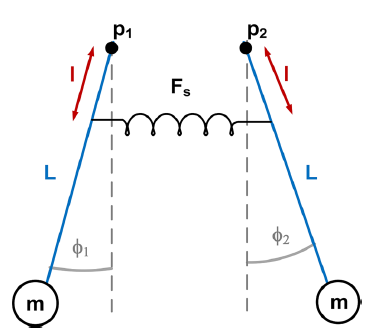
\includegraphics[width = 8 cm]{images/coupledpendula set up.png}
    \caption{The set up of the coupled pendula system.\citep{lab_note} \label{fig 1}}
\end{figure}
\begin{tikzpicture}
    \draw [thick,dash dot] (0,0) -- (9,0);
\end{tikzpicture}

\subsubsection{First Normal Mode}
The first normal mode of the coupled pendula system, is also known to be the in-phase oscillation mode. Is said to be when the two pendula are oscillating with the identical amplitude and frequency with no phase difference (\citeauthor{Taylor}, 2005, p. 423).

Note that in this mode, the spring is not being compressed nor extended. Therefore the spring have no contribution to the motion of the pendula. These two pendula will now have the same equation of motion which is identical to a single pendulum oscillating by itself. The equation of motion is
\begin{equation}
    \phi_1(t) = \phi_2(t) = \phi_{\text{max}} \cos (\omega_n t). \label{eq1}
\end{equation}
Where $\phi_{\text{max}}$ denotes the maximum amplitude of the pendula (note that both pendula have the same maximum amplitude), and $\omega_n$ denotes the natural \textbf{\emph{angular frequency}} of the system which is simply
\begin{equation}
    \omega_n = \sqrt{\frac{g}{L}}. \label{eq2}
\end{equation}

Note that the uncertainty of $\omega_n$ can be obtained by taking the Taylor expansion around zero, namely
\begin{equation}
    \Delta \omega_n = \sqrt{\left(\frac{\text{$\Delta $L} \sqrt{g}}{2 L^{3/2}}\right)^2+\left(\frac{\text{$\Delta $g}}{2 \sqrt{g L}}\right)^2}. \label{eq3}
\end{equation}

\begin{tikzpicture}
    \draw [thick,dash dot] (0,0) -- (9,0);
\end{tikzpicture}

\subsubsection{Second Normal Mode}
In the second normal mode, the pendula are oscillating with the same frequency and amplitude but they are perfectly out of phase (There is exactly $\pi$ radians difference between them). The equation of motions in this mode is now (\citeauthor{Taylor}, 2005, p. 425)
\begin{align}
    \phi_1(t) &= \phi_{\text{max}} \cos (\omega_o t)\\
    \phi_2(t) &= -\phi_{\text{max}} \cos (\omega_o t).
\end{align} 
With 
\begin{equation}
    \omega_o = \sqrt{\omega_n^2 + \frac{2kl^2}{mL^2}}, \label{eq6}
\end{equation}
and I obtained the uncertainty in similar fashion to the method used in obtaining eq. \ref{eq3}. Please refer to eq. \ref{eq7} in the \textbf{Long Equation} section for the uncertainty of $\omega_o$.

Unlike the first normal mode, the spring will contribute to the equation of motion in the second mode since it is being extended and compressed. Upon comparing eq. \ref{eq2} to eq. \ref{eq6}, it is obvious that 
$$\omega_o \ge \omega_n.$$
\begin{tikzpicture}
    \draw [thick,dash dot] (0,0) -- (9,0);
\end{tikzpicture}

\subsubsection{The Beat Mode}
In this system, any oscillations between the two normal modes are a linear combination of the normal modes (they are also called the eigenstates which makes sense), and one interesting case is when the two combination contributes the same amount (imagine this as the mid point between two normal modes). And this is called the beat mode. The equation of motions governing this mode are 
\begin{align}
    \phi_1(t) &= \frac{\phi_{\text{max}}}{2} (\cos(\omega_o t) + \cos(\omega_n t))\\
    \phi_2(t) &= -\frac{\phi_{\text{max}}}{2} (\sin(\omega_o t) - \sin(\omega_n t)).
\end{align}
\par\noindent\rule{\linewidth}{0.4pt}

\section{Method}
Firstly, the spring constant is measured using a number of weights. The spring is first place horizontally on the table to determined the equilibrium position (without it being affected by its own weight). Then, the changed of length are taken from each time a mass is added on the spring when it is hung vertically. The data are recorded, and to determined the spring's constant $k$. A linear regression model from SciPy\cite{2020SciPy-NMeth} is used. Where the slope of the regression model is said to be the spring constant with the standard error of the regression model being the uncertainty in the spring's constant.

Two identical pendula are set up along side of each other. The spacing between the connecting rods of the pendula are adjusted to be the equilibrium position of the spring we are using. A piece of specialised equipment is used to record the amplitude as voltages and time for both of the pendula. The sampling interval is set to be 0.005 seconds. In this experiment, three different position for the spring's placement $l$ is used mainly 0.6, 0.4 and 0.2 metres. 



























\bibliographystyle{agsm}
\bibliography{cp.bib}
%%%%%%%%%%%%%%%%%%%%%%%%%%%%%%%%%%%%%%%%%%%%%%%%%
\onecolumngrid
\newpage
\appendix
\section{Appendix}
\section{Long Equations}\label{LE}
\begin{equation}
    \begin{split}
        \Delta \omega_o = \Biggl\{\frac{\text{$\Delta $l}^2 k^2 l^2}{L^4 m^2 \left(\frac{g}{L}+\frac{k l^2}{L^2 m}\right)}+\frac{\text{$\Delta $m}^2 k^2 l^4}{4 L^4 m^4 \left(\frac{g}{L}+\frac{k l^2}{L^2 m}\right)}&+\frac{\text{$\Delta $k}^2 l^4}{4 L^4 m^2 \left(\frac{g}{L}+\frac{k l^2}{L^2 m}\right)}+\\
        &\frac{\text{$\Delta $g}^2}{4 L^2 \left(\frac{g}{L}+\frac{k l^2}{L^2 m}\right)}+\frac{\text{$\Delta $L}^2 \left(-\frac{g}{L^2}-\frac{2 k l^2}{L^3 m}\right)^2}{4 \left(\frac{g}{L}+\frac{k l^2}{L^2 m}\right)}\Biggr\}^{1/2} \label{eq7}
    \end{split}
\end{equation}
\subsection{Experiment Data and Source Codes}
For the experiment data and the source code please visit this \href{https://github.com/jojounderscorejo/CheatSheetRepo/tree/main/Otherthings/PHYS2113%20CP%20LAB}{\textbf{link}}.

\subsection{Figures}




\end{document}